\documentclass[10pt,aspectratio=169,handout]{beamer}

\usepackage[utf8]{inputenc}
\usepackage[ngerman]{babel}
\usepackage{utopia}
\usetheme{Darmstadt}
\usecolortheme{default}
\usepackage{xcolor}
\usepackage{graphicx}
\usepackage{amsmath}
\usepackage{amsthm}
\usepackage{amssymb}
\usepackage{amsfonts}
\usepackage{mathtools}
\usepackage{dsfont}
\usepackage{hyperref}
\usepackage[most]{tcolorbox}
\usepackage{tikz}
\usepackage{adjustbox}
\usepackage{mathrsfs}
\usepackage{minted}
\usetikzlibrary{cd}
\usetikzlibrary{positioning}
\usetikzlibrary{calc}
\usetikzlibrary{arrows.meta}
\setbeamertemplate{theorems}[numbered]
\setbeamertemplate{navigation symbols}{}
\newtranslation[to=ngerman]{Theorem}{Satz}
\def\C{\mathbb{C}}
\def\R{\mathbb{R}}
\def\Q{\mathbb{Q}}
\def\N{\mathbb{N}}
\def\Z{\mathbb{Z}}
\def\cA{\mathcal{A}}
\definecolor{LightGray}{gray}{0.9}


\begin{document}

\title{Principles of Machine Learning: Exercise 1}
\date{06.11.2023}
\author{Alina Pollehn (3197257), Julian Litz (3362592), Manuel Hinz (3334548)\\Felix Göhde (3336445), Felix Lehmann (3177181), Caspar Wiswesser (3221493) \\Adrian Köring (3347785), Greta Günther (3326765), Linus Mallwitz (3327653)\\ Name 10-11}

\begin{frame}
    \maketitle
\end{frame}

\section{Exercise 1.2}

\begin{frame}
    \frametitle{test}
    %\inputminted[bgcolor=LightGray]{python}{tmp.py}
\end{frame}


\section{Exercise 1.3}

\begin{frame}
    \frametitle{Fractal dimensions}

    \begin{enumerate}
        \item Binarize the image
        \item Partition the image into $2^l$ boxes for $l=1,\dots,L-2$,
        \item Calculate the fractal dimension using linear regression \[D\cdot \log\left(\frac{1}{s_l}\right)+b=\log(n_l)\] 
    \end{enumerate}    
    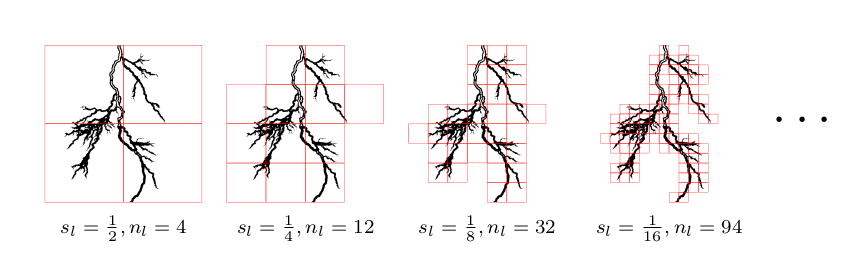
\includegraphics[scale=0.4]{images/boxes.png}

\end{frame}

\begin{frame}
    \frametitle{Implementation: Box counting}
    \inputminted[bgcolor=LightGray,fontsize=\small]{python}{box_counting.py}
\end{frame}

\begin{frame}
    \frametitle{Implementation: Calculating the fractal dimension}
    \inputminted[bgcolor=LightGray,fontsize=\small]{python}{get_slope.py}
    where np.vander generates the Vandermonde matrix
    \[V=\begin{bmatrix}
        1 & \log(2^1)^1\\
        1 & \log(2^2)^1\\
        \vdots & \vdots \\
        1 & \log(2^{L-2})^1
    \end{bmatrix}\]
\end{frame}

\begin{frame}
    \frametitle{Results}

    \begin{minipage}{0.45\textwidth}
        \begin{enumerate}
            \item Fractal dimension\begin{itemize}
                \item Tree: $\approx 1.846$
                \item Lighting: $\approx1.493$
            \end{itemize}
            \item The fractal dimension of the image ``lighting.png'' is higher
        \end{enumerate}
    \end{minipage}
    \begin{minipage}{0.45\textwidth}
        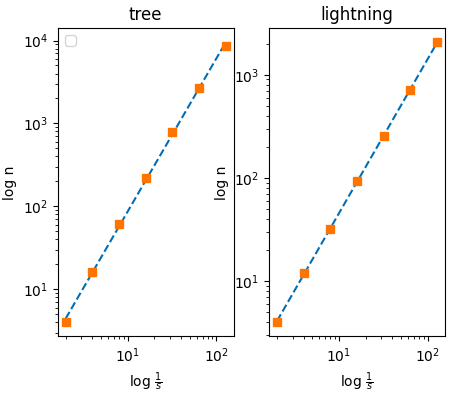
\includegraphics[scale=0.4]{images/plots.png}
    \end{minipage}
\end{frame}

\begin{frame}
    \frametitle{Learnings}
    \begin{enumerate}
        \item Fractal dimensions
        \item Fractal dimensions as a least squares problem using box counting
        \item Application of least squares to a wider class of problems
    \end{enumerate}
\end{frame}

\end{document}
